\documentclass[12pt]{report}

% includes
\usepackage{geometry}           % page size
\usepackage[utf8]{inputenc}     % encoding
\usepackage{palatino}           % font
\usepackage[english]{babel}    % language
\usepackage{graphicx}           % images
\usepackage{indentfirst}        % indentation
\usepackage[nottoc]{tocbibind}  % table of contents style
\usepackage[unicode]{hyperref}  % references from the table of contents
\usepackage{float}
\usepackage{listings}
\usepackage{enumitem}

% includes options
\geometry{  a4paper,            % scientific thesis standard
            left=3cm,
            right=2cm,
            top=2cm,
            bottom=2cm,
 }
\graphicspath{{images/}}        % path where the images are located
\setlength{\parindent}{1cm}     % paragraph indentation

% other options
\linespread{1.5}                % space between lines
\renewcommand*\contentsname{Contents}    % table of contents name

\usepackage{color}
\definecolor{jsComment}{RGB}{185, 185, 185}
\definecolor{jsKeyword}{RGB}{151, 97, 155}
\definecolor{jsString}{RGB}{136, 158, 26}

\lstdefinelanguage{JavaScript}{
  keywords={break, case, catch, continue, debugger, default, delete, do, else, false, finally, for, function, if, in, instanceof, new, null, return, switch, this, throw, true, try, typeof, var, void, while, with, await, async, from, const, let},
  morecomment=[l]{//},
  morecomment=[s]{/*}{*/},
  morestring=[b]',
  morestring=[b]",
  ndkeywords={class, export, boolean, throw, implements, import, this},
  keywordstyle=\color{jsKeyword}\bfseries,
  ndkeywordstyle=\color{jsKeyword}\bfseries,
  identifierstyle=\color{black},
  commentstyle=\color{jsComment}\ttfamily,
  stringstyle=\color{jsString}\ttfamily,
  sensitive=true
}

\definecolor{YAMLcolonstyle}{RGB}{200, 200, 200}
\definecolor{YAMLkeystyle}{RGB}{69, 126, 175}
\definecolor{YAMLvaluestyle}{RGB}{136, 158, 26}

\newcommand\YAMLcolonstyle{\color{black}\mdseries}
\newcommand\YAMLkeystyle{\color{YAMLkeystyle}\bfseries}
\newcommand\YAMLvaluestyle{\color{YAMLvaluestyle}\mdseries}

\makeatletter

% here is a macro expanding to the name of the language
% (handy if you decide to change it further down the road)
\newcommand\language@yaml{yaml}

\expandafter\expandafter\expandafter\lstdefinelanguage
\expandafter{\language@yaml}
{
  keywords={true,false,null,y,n},
  keywordstyle=\color{darkgray}\bfseries,
  basicstyle=\YAMLkeystyle,                                 % assuming a key comes first
  sensitive=false,
  comment=[l]{\#},
  morecomment=[s]{/*}{*/},
  commentstyle=\color{purple}\ttfamily,
  stringstyle=\YAMLvaluestyle\ttfamily,
  moredelim=[l][\color{orange}]{\&},
  moredelim=[l][\color{magenta}]{*},
  moredelim=**[il][\YAMLcolonstyle{:}\YAMLvaluestyle]{:},   % switch to value style at :
  morestring=[b]',
  morestring=[b]",
  literate =    {---}{{\ProcessThreeDashes}}3
                {>}{{\textcolor{red}\textgreater}}1     
                {|}{{\textcolor{red}\textbar}}1 
                {\ -\ }{{\mdseries\ -\ }}3,
}

% switch to key style at EOL
\lst@AddToHook{EveryLine}{\ifx\lst@language\language@yaml\YAMLkeystyle\fi}
\makeatother

\newcommand\ProcessThreeDashes{\llap{\color{cyan}\mdseries-{-}-}}

% the document content
\begin{document}
    % macros (global)
    \newcommand{\university}    {"Alexandru-Ioan Cuza" University of Iasi}
\newcommand{\universityg}   {Universității "Alexandru-Ioan Cuza" din Iași} % genitive
\newcommand{\faculty}       {Faculty of Computer Science}
\newcommand{\facultyg}      {Facultății de informatică} % genitive
\newcommand{\speciality}    {informatică}
\newcommand{\promotion}     {2021}                                  %<---------

\newcommand{\thesistype}    {Bachelor Thesis}
\newcommand{\thesistitle}   {Think-In - A virtual conference application}    %<---------

\newcommand{\authorlast}    {Crisan}                               %<---------
\newcommand{\authorfirst}   {Mihai}
\newcommand{\authornamefl}  {\authorfirst \space \authorlast} % first name first
\newcommand{\authornamelf}  {\authorlast \space \authorfirst} % last name first
\newcommand{\authorbirth}   {15 october 1999}                      %<---------
\newcommand{\authoraddress} {România, jud. Galaţi, sat. Matca (com. Matca), Strada Morii, nr. 74} %<---------
\newcommand{\authorcnp}     {1991015226702}                         %<---------

\newcommand{\session}       {june-july, 2021}                       %<---------
\newcommand{\coordinator}   {Prof. Dr. Alboaie Lenuţa}               %<---------

\newcommand{\dottedline}    {............................}
    
    % front-matter
    \pagenumbering{gobble}
    
    \input{front/cover}
    \input{front/titlepage}
    \input{front/declaration1}
    \input{front/declaration2}
    
    % table of contents
    \tableofcontents
    
    % chapters
    \setcounter{page}{1}
    \pagenumbering{arabic}
    
    \input{chapters/motivation}
    \chapter*{Introduction} 
\addcontentsline{toc}{chapter}{Introduction}

The proposed solution to the previously mentioned problems has the name \textbf{Think-In}, and is a web application where virtual conferences or events can be held with the purpose of networking.
Having mentioned the two below issues, the \textbf{general purpose} of the application is to help people connect and network, therefore the users will expand their professional relationships and find new opportunities:

\begin{itemize}
    \item 
An issue that can appear in conferences of bigger sizes because of the diversity of the attenders, which other existent applications don't solve, is the \textbf{language barrier}. \textbf{Think-In} solves this issue as messages sent across the conference are translated in real-time in the user's native language or any other language the user desires. This feature can bring people together from all around the world as there are no communication bounds.
    \item
An inherent problem to real world conferences or events is that you don't know many of the people who attend, therefore the \textbf{Think-In} users have the option to provide more information about themselves such as an avatar, their job title and links to their social media accounts so they can be easily discovered and engaged with.
\end{itemize}

As a response to the disadvantages stated at the end of the previous chapter, \textbf{Think-In} is platform agnostic so the user can use the application no matter what device it is accessed from, it was designed to be blazing fast and very easy to use. In contrast to the aforementioned desktop applications, it is a web application, therefore the developers don't have to take care of how updates are brought to the users because everytime the user reloads the page the newest version of the application is used.

From a technical point of view, the application's \textbf{frontend} is built using the Next.js\footnote{No configuration React framework: \href{https://nextjs.org/}{https://nextjs.org/}} React\footnote{JavaScript library for building user interfaces: \href{https://reactjs.org/}{https://reactjs.org/}} framework and has a JAMstack\footnote{\href{https://jamstack.org/}{https://jamstack.org/}} architecture, the pages are built at deploy time and they are stored in a S3\footnote{AWS' object storage service: \href{https://aws.amazon.com/s3/}{https://aws.amazon.com/s3/}} bucket as a static website, from there on they are served from the CloudFront\footnote{AWS' CDN service: \href{https://aws.amazon.com/cloudfront/}{https://aws.amazon.com/cloudfront/}} CDN\footnote{Content Distribution Network}. This setup ensures a very fast TTFB\footnote{Time To First Byte} since there are no round trips to the server in order to render the page and the files required for the web page are fetched from one of the CDN's proxy servers, which, as a consequence of being close to the user, ensure fast file retrieval. The \textbf{backend} relies on a Socket.IO\footnote{Real-time communication library which uses WebSockets or HTTP as a fallback: \href{https://socket.io/}{https://socket.io/}} server ensuring the fastest communication possible when stage interactions happen or when messages are sent, as well as an AWS API Gateway\footnote{API management tool \href{https://aws.amazon.com/api-gateway/}{https://aws.amazon.com/api-gateway/}} that centralizes access to Lambda\footnote{AWS' event-driven serverless compute service: \href{https://aws.amazon.com/lambda/}{https://aws.amazon.com/lambda/}} functions, which act as a REST API when they are triggered by HTTP events. TypeScript\footnote{JavaScript superset language that adds static typing: \href{https://www.typescriptlang.org/}{https://www.typescriptlang.org/}} was the language of choice all around the application stack, this was motivated by the fact that the frontend had to be written in JavaScript and the opportunity to reuse code in the backend was hard not to take. Additionally, TypeScript brings static typing to JavaScript, that has proved to be extremely helpful in eliminating type errors as well as simplifying the developing experience thanks to type hints povided by modern IDEs. In order to simplify the deployment of the application, DevOps practices such as CI/CD\footnote{Continuous Integration and Continuous Deployment} and IaC\footnote{Infrastructure as Code} have been adopted.

%TODO: metodologia folosită, structura lucrării (titlul capitolelor și legătura dintre ele).
    \chapter*{Contributions} 
\addcontentsline{toc}{chapter}{Contributions}

While the concept of virtual conferences and events is not new, I have attempted to streamline the user interactions in order to provide quick access to what the attenders want. I have analyzed other existent solutions, borrowed their strongest points and tried to overcome what I thought was lacking. I tried to rethink the business logic so smoother experiences can be had. Apart from thinking of an improved business logic, I also was in the position of choosing the best application architecture that will fit to the proposed business rules.

The combination of the ideas and the used cloud services have brought \textbf{Think-In} to an actual tangible product that can be accessed by anyone in the world, additionally, the used technologies and services allow for a very easy extension so that the application can fully scale horizontally. The application can be used by any kind of company since no technical skills are required in order to setup new stages.

I would like to thank my coordinator \textbf{\coordinator} because even from the very beginning she advised me what technologies I should learn and has been alongside me in the decision of the thesis theme and what features are worth adding.
    
    \chapter{Business logic}

At its most basic form, conferences are meant to be a formal meeting of people with a shared interest, it is meant to be an area where information is exchanged and people get to know each other. Without much thought, we realize that people at conferences are divided into two groups: organizers and visitors; thus, there must be a slight distinction between the two.

% From now on we will refer to organizers as \textbf{admins} and visitors as \textbf{attendees}.

\section{Attendee user flow}

In this subchapter we will analyze what steps an attendee has to go through in order to start using the application, we will start from the very beginning and we will be going into the details of certain features as well as how these can be used. For the purpose of completeness as many steps as possible will be described and images will be used to visualize the said ideas.

\subsection{Visiting the website and signing up}
By visiting the website for the first time we will be greeted with a page where the attendee is prompted to authenticate before using the application.

\begin{figure}[H]
	\includegraphics[width=\textwidth,keepaspectratio]{images/business_logic/main_page_not_signed_in.png}
	\caption{Website main page when not signed in.}
	\label{figure:website-main-page}
\end{figure}

An attendee has to have an identity, therefore signing in is necessary before using the application. Upon clicking the \textit{Sign In} button located at the right side of the page header the user is presented with the option of signing in through a third party (social sign in with Google in this case) which significantly speeds up the signing up process, or the more traditional option of using an account created specifically for \textbf{Think-In}.

\begin{figure}[H]
	\includegraphics[width=\textwidth,keepaspectratio]{images/business_logic/sign_in_page.png}
	\caption{Website sign in page.}
	\label{figure:website-sign-in-page}
\end{figure}

If the user signs in through an identity provider then he is redirected to the main page (shown in the next subsection), otherwise he has to go to the sign up page by clicking the \textit{Sign Up} button.

\begin{figure}[H]
	\includegraphics[width=\textwidth,keepaspectratio]{images/business_logic/sign_up_page.png}
	\caption{Website sign up page.}
	\label{figure:website-sign-up-page}
\end{figure}

The user has the choice of selecting an avatar and has to provide the information labeled in the above picture. In case the user did not pick an avatar, an identicon\footnote{\href{https://en.wikipedia.org/wiki/Identicon}{https://en.wikipedia.org/wiki/Identicon}} is generated and is used as the avatar. Upon signing up, the user has to confirm the just created account by following a link sent to the entered email address.

\begin{figure}[H]
	\includegraphics[width=\textwidth,keepaspectratio]{images/business_logic/sign_up_email_confirmation.png}
	\caption{Email confirmation showcasing HTML email.}
	\label{figure:email-confirmation}
\end{figure}

Upon confirming the account and signing in, the user is redirected to the main page.

\subsection{Main page}

The main page is where the users gather and communicate as well as view the media made available by a certain stage.

\begin{figure}[H]
	\includegraphics[width=\textwidth,keepaspectratio]{images/business_logic/main_page_signed_in_top.png}
	\caption{Top part of main page when signed in.}
	\label{figure:website-main-page-top}
\end{figure}

In the top part of the main page there is a horizontally scrolling list of stages from which the user can choose to join, every stage has attached a title, subtitle, an external link to the entity representing the stage, a description as well as two actions, \textit{Join Stage} and \textit{View Video}. The first action changes the stage, while the second one gives direct access to the video made available by the entity representing the stage.

\begin{figure}[H]
	\includegraphics[width=\textwidth,keepaspectratio]{images/business_logic/main_page_signed_in_center.png}
	\caption{Center part of main stage when signed in.}
	\label{figure:website-main-page-center}
\end{figure}

In the center of the main page is the actual stage where users can move their character by simply clicking to the desired location, here the currently present attendees can be seen, in this case \textit{John Doe} and \textit{Crisan Mihai}. As seen in the image above, an attendee is represented by its name and avatar, the current user has a slightly larger character and a green outline instead of grey. The screenshot is taken from the perspective of the user \textit{Crisan Mihai}. In the top part of the stage a looped video is playing, upon clicking it a smooth animation will bring the user closer to the playing media.

\begin{figure}[H]
	\includegraphics[width=\textwidth,keepaspectratio]{images/business_logic/main_page_signed_in_center_video.png}
	\caption{Media playing in the stage.}
	\label{figure:website-main-page-playing-media}
\end{figure}

When the user doesn't want to see anymore of the video, he simply clicks again on it and is taken back to the default stage view. In the default stage view, the user can click on an attendee's avatar in order to get more information about him.

\begin{figure}[H]
	\includegraphics[width=\textwidth,keepaspectratio]{images/business_logic/main_page_signed_in_attendee_dialog.png}
	\caption{Attendee dialog box.}
	\label{figure:website-attendee-dialog-box}
\end{figure}

In the above screenshot we have clicked on \textit{John Doe}'s avatar and a dialog has popped up showing us in addition to his name and avatar which we already knew, his job title (iOS Engineer) and various contact links from where we can gather more information about him. Furthermore, there is a \textit{Message} action that allows us to message \textit{John Doe}, by clicking it a new chat is opened and messages can be sent.

\begin{figure}[H]
	\includegraphics[width=\textwidth,keepaspectratio]{images/business_logic/main_page_signed_in_chat.png}
	\caption{Messaging an attendee, perspective of the sender.}
	\label{figure:website-attendee-messaging-sender}
\end{figure}

The above screenshot is from the perspective of \textit{Crisan Mihai}, what is to be observed is that the messages are translated in your native language, as it is visible in the screenshot below from \textit{John Doe}'s perspective.

\begin{figure}[H]
	\centering
	\includegraphics[width=0.5\textwidth,keepaspectratio]{images/business_logic/main_page_signed_in_chat_translated.png}
	\caption{Messaging an attendee, perspective of the receiver which has a different language set than the language of the messages.}
	\label{figure:website-attendee-messaging-receiver}
\end{figure}

Because \textit{John Doe} has selected Romanian as his language, all the messages he sees will be translated into Romanian.

Apart from the just described private chat messages that can be sent only between a pair of users, there are two other types of chats: 
\begin{itemize}
	\item Global chat - in this chat the messages are visible to everyone and it is accessible despite of the selected stage
	\item Stage chat - there is one stage chat for each stage available, i.e. one chat per stage which is only accessible when the user is in that stage
\end{itemize}

\subsection{Profile page}

As shown in the previous subsection, \textit{John Doe} has made available links to his social media but nowhere in the sign up process for instance he was asked to provide this information. There is a page where a user can add data about himself, change the avatar or data he has already provided, the language he speaks in and wants to see the messages in. Furthermore, in this same page a user has the option of changing his email or password as well as deleting his account. A screenshot can be seen below.

\begin{figure}[H]
	\centering
	\includegraphics[width=\textwidth,keepaspectratio]{images/business_logic/profile_page.png}
	\caption{Overview of the profile page.}
	\label{figure:website-profile-page}
\end{figure}

It is worth noting that in the case where the user has signed in through a third party, some of the attributes and actions won't be available, to be more explicit the following are not open to change:

\begin{itemize}
	\item Avatar, first name and last name - the data used here are provided by the third party identity provider, if they are to be changed, they have to be changed at the identity provider level
	\item Change email and password actions - there was no email or password set in the first place, therefore there is nothing that can be changed
\end{itemize}

\section{Organizer user flow}

The organizer/admin of the application has the same functionalities as a normal attendee plus the capability of adding, updating or deleting a stage. These functionalities are only visible to organizers/admins and are reachable from the Profile page, which was detailed in the previous section's last subsection. 

The page where a new stage can be added is shown below, media such as image and video can be drag and dropped into the corresponding areas.

\begin{figure}[H]
	\centering
	\includegraphics[width=\textwidth,keepaspectratio]{images/business_logic/stages_add.png}
	\caption{Add stage page.}
	\label{figure:add-stage-page}
\end{figure}

The page where a stage can be edited is very similar to the the one where a stage is added, the difference is that the input fields are filled based on the stage selected for editing. What's more is a delete stage action which is self-explanatory.

\begin{figure}[H]
	\centering
	\includegraphics[width=\textwidth,keepaspectratio]{images/business_logic/stages_edit.png}
	\caption{Edit stage page.}
	\label{figure:edit-stage-page}
\end{figure}

    \chapter{Adopted methodology and techniques}

Every software application is developed using certain paradigms and methodologies, \textbf{Think-In} is no different. In this chapter the choice of the chosen methodology will be explained as well as other used techniques that aided in the development process.

\section{Analyzing methodologies}
Rationally, before making any choice, I analyzed popular software development methodologies and frameworks that have been proven to work in the industry in order to see how they fit to my particular use case:

\begin{description}[style=unboxed, labelwidth=\linewidth]
	\item[Waterfall]
	By definition the waterfall model restricts going back to previous phases and this was very troublesome because for instance it was extremely hard to establish all the requirements beforehand. If for example a new idea appeared in the meantime it would have not been easy to introduce it as a result of how strongly structured this model is. Perhaps a modified waterfall could alleviate this issue but a better model can handle it more effectively.
    \item[Scrum]
	Although extremely popular and effective, the scrum methodology is more destined towards teams that consists of a couple or more members. Since the thesis is intended to be done by a single student this was not the best fit.
	\item[Extreme Programming (XP)]
	The requirements of the application would be changing frequently and extreme programming would accomodate for these changes. The practice of having numerous short releases sounded beneficial because new requirements could be observed once we have a working version of the product.
\end{description}

\section{Picking a methodology}

\
Considering my case and the above examination it became clear that Extreme Programming was the better option among them. Along the mentioned advantages of XP found above, XP is based on the Agile paradigm and the values of Agile were also found to be appealing. Standout practices of this framework that were used were the following:

\begin{itemize}
	\item Planning game - Informal explanations such as user stories were used to represent requirements. After writing and estimating the stories, they were sorted by their priority in the sense of the higher the business value they brought the higher the priority. After this operation, the ones with higher priority were chosen to be worked on first. Example of the user stories used:

	\begin{itemize}
		\item As an attendee I want to move my avatar in the stage by mouse click.
		\item In order to get to use the application faster as a user, I can login with a third party instead of creating an account.
		\item As a user I want to private message others.
		\item In order for other attendees to recognize me, I want to change my avatar.
		\item As an attendee I want to switch between stages, so that I can get to know more people and acquire knowledge from the other stages.
		\item As a user I want to get more information about another attender.
	\end{itemize}
	
	\item Design improvement - There was no hesitance in refactoring code or changing the architecture in favor of a more simple implementation.
	\item Small releases - By using the released application it was easier to come up with new improvements and suggestions, therefore there were frequent releases.
	\item Continuous integration - A Continuous Integration and Continuous Deployment pipeline was setup so that the application could be deployed faster and easier.
	\item Coding standard - Code conventions were established and enforced by tools (i.e. ESLint\footnote{\href{https://eslint.org/}{https://eslint.org/}} in this case) in order to eliminate problematic patterns and to keep a consistent style across all the source code. To reduce code comments that are hard to be maintained, an effort was put into writing self-documenting\footnote{\href{https://en.wikipedia.org/wiki/Self-documenting\_code}{https://en.wikipedia.org/wiki/Self-documenting\_code}} code.
	\item Simple design - Whenever there was a simpler way to achieve the same functionality the code or architecture was refactored.
\end{itemize} 
\
As a short conclusion, simplicity was valued throughout the whole project. I think that the conventions I opted for throughout the whole project will make it easier to be maintained over time. Moreover, the conventions used will also make it easier for newcomers to the project to understand the codebase faster.
\section{Elaborating on requirements}

Where additional specifications of a requirement were needed, I have relied on using text based \textbf{use cases}. For example, in Table \ref{table:change-profile-picture-use-case} we can see the use case I have written before implementing the functionality of changing a user's profile picture.

\begin{table}
	\centering

	\begin{tabular}{ | p{3.2cm} | p{11cm} | }
	 	\hline 
		\textbf{Name} & Change profile picture. \\
		\hline
		\textbf{Description} & The user can change its profile picture so its avatar (when browsing the stage) is more recognizable. \\
		\hline
		\textbf{Actors} & User and system. \\
		\hline
		\textbf{Trigger} & On the user profile page, the user presses the image indicating his current avatar. \\
		\hline
		\textbf{Preconditions} & The user is logged in. \\
		\hline
		\textbf{Postconditions} & The user will have a new profile picture. \\
		\hline
		\textbf{Basic flow} & \begin{enumerate}[topsep=1em,parsep=-.5em]
			\item User goes to profile page.
			\item User clicks on picture image.
			\item User uploads image from file system.
			\item User sees preview of his new profile picture before submitting changes.
			\item User clicks \textit{Save Changes}.
		\end{enumerate}} \\
		\hline
	\end{tabular}	

	\caption{Change profile picture use case.}
	\label{table:change-profile-picture-use-case}
\end{table}

I also wanted to clarify how an attendee can join a stage because that wasn't clear at first thought either, that use case is visible in Table \ref{table:join_stage_use_case}.

\begin{table}
	\centering

	\begin{tabular}{ | p{3.2cm} | p{11cm} | }
		\hline
		\textbf{Name} & Join a stage. \\
		\hline
		\textbf{Description} & An attendee joins a stage. \\
		\hline
		\textbf{Actors} & User and stage. \\
		\hline
		\textbf{Trigger} & User clicks the \textit{Join Stage} button of the stage he wants to join.  \\
		\hline
		\textbf{Preconditions} & The user is logged in and at the index page. \\
		\hline
		\textbf{Postconditions} & The page will refresh, showing the contents of the selected stage. \\
		\hline
		\textbf{Basic flow} & \begin{enumerate}[topsep=1em,parsep=-.5em]
			\item The user is logged in at the index page where there will be a list of stages to choose from.
			\item User clicks on the \textit{Join Stage} button of the stage he wants to join.
			\item The page will reload with the stage changed.
		\end{enumerate}} \\
		\hline
	\end{tabular}	

	\caption{Join a stage use case.}
	\label{table:join_stage_use_case}
\end{table}

I wanted to enhance the possibility of getting more information about a user, therefore I made sure there is a way to access more data about an attendee from anywhere he is mentioned. There are three ways in total where a user pops up: from the stage, from an opened chat with that user, or from a message the user wrote. Writing a use case helped in deciding how all of it is going to work in more detail. This use case is shown in Table \ref{table:contact_user_use_case}.

\begin{table}
	\centering
	\begin{tabular}{ | p{3.2cm} | p{11cm} | }
		\hline
		\textbf{Name} & Get more information about a user. \\
		\hline
		\textbf{Description} & While using the application the user sees somebody who he would like to get more information about. \\
		\hline
		\textbf{Actors} & Current user and target user (the user whose information wants to be seen)  \\
		\hline
		\textbf{Trigger} & The current user clicks on the target user avatar. \\
		\hline
		\textbf{Preconditions} & The user is logged in and at the index page. \\
		\hline
		\textbf{Postconditions} & A dialog box will pop up containing more information about the target user.\\
		\hline
		\textbf{Basic flow} & \begin{enumerate}[topsep=em,parsep=-.5em]
			\item The current user is looking at the stage and a certain user (Target user in this case) attracts his attention.
			\item The current user clicks on the target user's avatar.
			\item A dialog box pops up with information regarding the target user.
		\end{enumerate}} \\
		\hline
		\textbf{Alternate flow 1} & \begin{enumerate}[topsep=0em,parsep=-.5em]
			\item The current user has been messaged by the target user and the current user wants to see more information about him.
			\item The current user clicks on the three vertical dots button alongside the target user's chat.
			\item The current user clicks on \textit{View Profile}
			\item A dialog box pops up with information regarding the target user.
		\end{enumerate} \\
		\hline
		\textbf{Alternate flow 2} & \begin{enumerate}[topsep=0em,parsep=-.5em]
			\item The current user sees a message in the chat from the target user and wants to see more information about him.
			\item The current user clicks on the avatar on the left side of the target user.
			\item A dialog box pops up with information regarding the target user.
		\end{enumerate} \\
		\hline
	\end{tabular}	
	
	\caption{Contact a user use case.}
	\label{table:contact_user_use_case}
\end{table}

    \chapter{Application infrastructure and architecture}

In this chapter I am going to talk about the services that \textbf{Think-In} relies on and why I chose them, afterwards I am going to talk about the application's architecture, used technologies and tools.

\section{Application infrastructure}

\textbf{Think-In} is supposed to be an application with people networking in mind, therefore allowing humans far away from each other to connect. Because of this, it had to be available to the public internet. Hosting the application on my own machine would have implied a lot of time spent on maintenance, implementation and let's not even mention the security nightmare that it would have been. The issue of scalability would have been impossible to solve as well. Quickly thereafter I realised that XaaS\footnote{Everything as a service: \href{https://en.wikipedia.org/wiki/As\_a\_service}{https://en.wikipedia.org/wiki/As\_a\_service}} offerings by cloud computing providers would solve the issues I would face and it would save a lot of time and energy, all while using robust and proven to work software.

\subsection{Choosing a main cloud platform to use}

During my research I have found Gartner\footnote{Research and advisory firm: \href{https://www.gartner.com/en}{https://www.gartner.com/en}} to have a great reputation and provide reliable reports on cloud computing service providers. As a result I chose to inspect their famous magic quadrants during which I have found a \textit{Magic Quadrant for Cloud Infrastructure and Platform Services}\footnote{\href{https://aws.amazon.com/blogs/aws/aws-named-as-a-cloud-leader-for-the-10th-consecutive-year-in-gartners-infrastructure-platform-services-magic-quadrant/}{https://aws.amazon.com/blogs/aws/aws-named-as-a-cloud-leader-for-the-10th-consecutive-year-in-gartners-infrastructure-platform-services-magic-quadrant/}}. Instinctively I would choose a provider with significant age in the field because if I were to face an issue then certainly I wouldn't be first one to do so and I would easily find a fix on the web. Moreover I would expect a cloud provider with experience to have well written documentation about their services, which, because I am a beginner, is essential to me. As a consequence I will consider only the very well known providers as an option.

In the top right quadrant for this specific report (corresponding to the leaders in this domain) I found three providers: Google, Microsoft and Amazon Web Services. All of them have a free offering so I went to research by using each one individually:

\begin{description}[style=unboxed, labelwidth=\linewidth]
	\item[Google Cloud Platform]
	Out of all three providers I found Google to have the best project organization, all created resources are within a logical entity (a project) and that would help me as a newcomer to not confuse resources. Moreover they have the most generous free tier. Unfortunately I found certain services not to work as good as others, for example their API Gateway seems to lack in features compared to the one provided by AWS, it was also hard to read event logs from Cloud Functions.
    \item[Microsoft Azure]
	I have found this platform to be more confusing than others, I also did not like the experience using the web console (e.g. horizontal scrolling), more than this I had trouble using the web console to upload a collection of files under a directory on their object storage service.
	\item[Amazon Web Services (AWS)]
	I "clicked" with the services provided by AWS more than any other cloud provider, they felt simple to use and packed with features. AWS has been available for more time than the other two and is very well established which for sure meant great documentation and lots of resources to learn from. One thing I found inferior compared to others was the organization of resources based on regions.
\end{description}

This being said, I chose Amazon Web Services as the main cloud provider.

\section{Application architecture}

Below is attached a simplified overview of the application's architecture, it can be used as a reference when we will go into more detail about the implementation.

\begin{figure}[H]
	\centering
	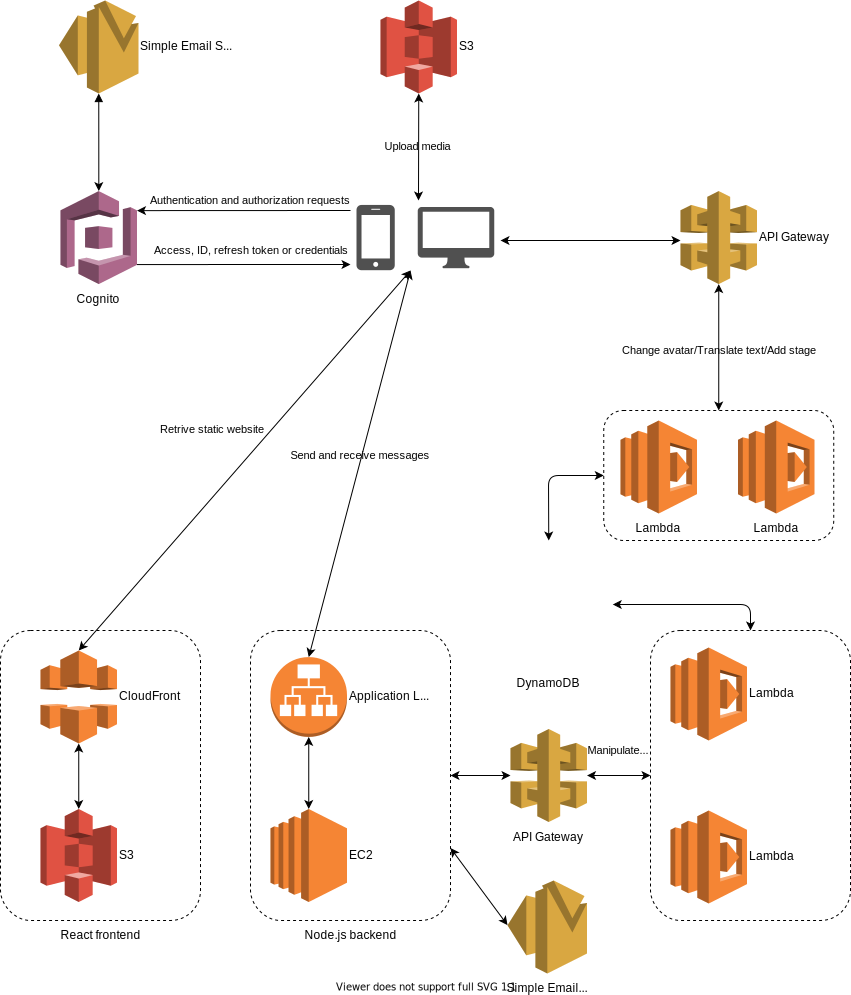
\includegraphics[width=\textwidth,keepaspectratio]{images/architecture/architecture.pdf}
	\caption{Application architecture.}
	\label{figure:application-architecture}
\end{figure}

Efforts were put into making the application scale as well as possible, this is why for instance the REST API was created from HTTP triggered Lambda functions, they scale to "infinity". Interesting aspects are that the API is accessed both client-side and server-side, everything that could be done from the client has been done from the client, however as we will see later some actions are only possible on the backend. The backend performs communication using websockets in order to ensure real-time message transmission.

Instead of creating an authentication system I relied that weight on AWS Cognito user pools\footnote{\href{https://docs.aws.amazon.com/cognito/latest/developerguide/cognito-user-identity-pools.html}{https://docs.aws.amazon.com/cognito/latest/developerguide/cognito-user-identity-pools.html}} so that I could easily manage user confirmation, password resets, changing email or other attributes and more without having to build that infrastructure myself. Moreover, Cognito was also used for providing temporary AWS credentials for certain services (e.g S3) so that the client could interact with these services directly.

\section{Continuous Integration and Continuous Deployment}

As talked about in the last chapter, values were found in having short and quick releases, therefore a pipeline that automates the process of deploying the application was set up. Below, in Figure \ref{figure:cicd}, is a diagram showcasing the flow of how the application is built.

\begin{figure}[H]
	\centering
	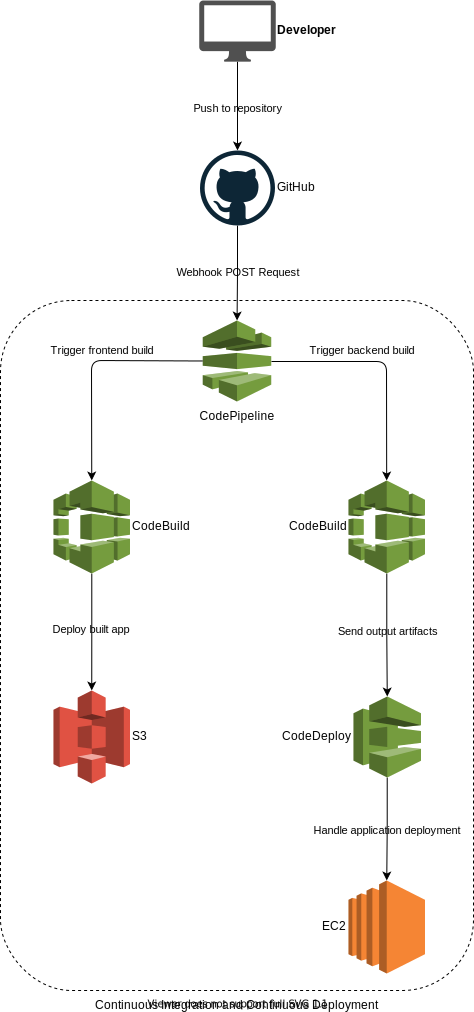
\includegraphics[width=.7\textwidth,keepaspectratio]{images/architecture/cicd.pdf}
	\caption{Continuous Integration and Continuous Deployment overview.}
	\label{figure:cicd}
\end{figure}

For those more familiar with CodePipeline, a screenshot of the pipeline from the AWS console is shown in Figure \ref{figure:codepipeline-cicd}.

\begin{figure}[H]
	\centering
	\includegraphics[width=\textwidth,keepaspectratio]{images/architecture/codepipeline-cicd.png}
	\caption{CodePipeline from AWS console.}
	\label{figure:codepipeline-cicd}
\end{figure}

Whenever a push to the GitHub repository is done, a webhook is triggered and GitHub sends a POST request to AWS that starts the pipeline. I set up the pipeline so that two parallel builds are started at once: the \textbf{frontend} and \textbf{backend} builds.

The code executed for the frontend build can be found in Figure \ref{figure:cicd-frontend-buildspec}. In the \textit{install} phase the npm\footnote{\href{https://www.npmjs.com/}{https://www.npmjs.com/}} package manager is installed in a non-interactive way (as a result of the \verb|--assume-yes| option) which is needed for installing the application's dependencies. Because all the source code is organized into a monorepo\footnote{\href{https://en.wikipedia.org/wiki/Monorepo}{https://en.wikipedia.org/wiki/Monorepo}}, in the \textit{pre\_build} phase the working directory has to be changed, in this case to the directory where the frontend application is. Next, on line 14, a clean install of the application's dependencies is done. In the \textit{build} phase I have abstracted the exporting of the application in a single npm script. After the \textit{build} phase is done, the output artifacts corresponding to the built application are put into a S3 bucket from where the CloudFront CDN will serve the static files to clients.

\begin{figure}[H]
\begin{lstlisting}[numbers=left,language=yaml]
version: 0.2
phases:
  install:
    runtime-versions:
      nodejs: 14.x
    commands:
      - apt --assume-yes update
      - apt --assume-yes install npm
    finally:
      - echo Install phase done.
  pre_build:
    commands:
      - cd app/FE
      - npm ci
    finally:
      - echo Prebuild phase done.
  build:
    commands:
      - npm run export
    finally:
      - echo Build phase done.
artifacts:
  base-directory: 'app/FE/out'
  files:
    - '**/*'
\end{lstlisting}
\caption{Frontend CodeBuild specification}
\label{figure:cicd-frontend-buildspec}
\end{figure}

On the other side, the code executed by CodeBuild for the backend build can be found in Figure \ref{figure:cicd-backend-buildspec}. The \textit{install} phase is the same as in the frontend build specification. Similar to the frontend, in the \textit{pre\_build} phase we change the working directory to where the backend app is and install the dependencies. The first command in the \textit{build} phase creates the environment file on the fly by retrieving the environment variables I have stored in AWS System Manager Parameter Store\footnote{Centralized place for keeping secrets/parameters: \href{https://aws.amazon.com/systems-manager/}{https://aws.amazon.com/systems-manager/}}. The next command builds the application, after which the output artifacts are passed on to CodeDeploy.

\begin{figure}[H]
\begin{lstlisting}[numbers=left,language=yaml]
version: 0.2
phases:
  install:
    runtime-versions:
      nodejs: 14.x
    commands:
      - apt --assume-yes update
      - apt --assume-yes install npm
    finally:
      - echo Install phase done.
  pre_build:
    commands:
      - cd app/BE/stage_server
      - npm ci
    finally:
      - echo Prebuild phase done.
  build:
    commands:
      - npm run create-env
      - npm run build
    finally:
      - echo Build phase done.
artifacts:
  base-directory: 'app/BE/stage_server'
  exclude-paths: 'src/**/*'
  files: '**/*'
\end{lstlisting}
\caption{Backend CodeBuild specification}
\label{figure:cicd-backend-buildspec}
\end{figure}

The artifacts are now in CodeDeploy's hands which has the specification shown in Figure \ref{figure:cicd-backend-appspec}. Lines 3-5 specify the path to where the artifacts will be put on the EC2 machine. Lines 7-12 attach shell scripts to different lifecycle events which are self-explanatory, now we will explore each script in detail.

\begin{figure}[H]
\begin{lstlisting}[numbers=left,language=yaml]
version: 0.0
os: linux
files:
  - source: /
    destination: /home/ubuntu/websocket-server/
hooks:
  ApplicationStop:
    - location: ./scripts/application-stop.sh
  BeforeInstall:
    - location: ./scripts/before-install.sh
  ApplicationStart:
    - location: ./scripts/application-start.sh
\end{lstlisting}
\caption{Backend CodeDeploy specification}
\label{figure:cicd-backend-appspec}
\end{figure}

The \textit{application-stop.sh} script (Figure \ref{figure:cicd-backend-appspec-application-stop}) is run for the \textit{ApplicationStop} lifecycle event, here we have to stop the previously running application. We store the process id of the running process in the \textit{pid} variable after which, if there was a process id found, the process is killed. Otherwise, corresponding to the case where there is no process id found, nothing happens.

\begin{figure}[H]
\begin{lstlisting}[numbers=left,language=bash]
#!/bin/bash
pid=`ps aux | grep "node out/index.js" | grep -v grep | tr -s " " " "
 | cut -d " " -f2`
# if string is not empty
if [ -n "${pid}" ]
then
    kill -9 $pid
    echo Killed process with pid $pid
else
    echo Found no process with pid $pid
fi
\end{lstlisting}
\caption{Backend CodeDeploy application stop script.}
\label{figure:cicd-backend-appspec-application-stop}
\end{figure}

Next up is the \textit{before-install.sh} script (Figure \ref{figure:cicd-backend-appspec-before-install}). This script simply clears the directory where the application is.

\begin{figure}[H]
\begin{lstlisting}[numbers=left,language=bash]
#!/bin/bash
rm -rf /home/ubuntu/websocket-server
mkdir /home/ubuntu/websocket-server
\end{lstlisting}
\caption{Backend CodeDeploy before install script.}
\label{figure:cicd-backend-appspec-before-install}
\end{figure}

Before this script is ran, the built files have been copied to the \textit{/home/ubuntu/websocket-server} directory. Finally we have the \textit{application-start.sh} script (Figure \ref{figure:cicd-backend-appspec-application-start}). We first navigate to the directory where the application is, we install its dependencies non-interactively and we create the environment file on the fly just like in the build phase. After this everything has been finished and we can start the application by running \textit{yarn start} which corresponds to the command below:

\begin{lstlisting}[language=bash]
nohup node out/index.js > stdout.log 2> stderr.log < /dev/null &
\end{lstlisting}

\begin{figure}[H]
\begin{lstlisting}[numbers=left,language=bash]
#!/bin/bash
cd /home/ubuntu/websocket-server
yarn install --non-interactive
node `dirname "$BASH_SOURCE"`/application-start-create-env.js
yarn start
\end{lstlisting}
\caption{Backend CodeDeploy application start script.}
\label{figure:cicd-backend-appspec-application-start}
\end{figure}

\section{REST API Deployment}

For managing the deployment of the REST API I have relied on Serverless\footnote{\href{https://www.serverless.com/}{https://www.serverless.com/}} framework, it has allowed me to easily deploy AWS resources such as Lambda functions, API Gateway and DynamoDB\footnote{Fast and flexible NoSQL database: \href{https://aws.amazon.com/dynamodb/}{https://aws.amazon.com/dynamodb/}}. For this I have used DevOps practices such as Infrastructure as Code for configuring the resources that are created.

Going further we're going to analyze the configuration code (Figure \ref{figure:iac-function-example}) for a Lambda function as an example. On line 2, we specify the path to the function that will be executed when this Lambda function is triggered. Line 4 to 11 indicate that this function is HTTP triggered whenever a \verb|GET| request is sent to \verb|/chats/{chatId}|, moreover it attaches an authorizer so only tokens created by AWS Cognito are approved. Lines 12-17 define the roles this function has, in this case it allows the \verb|dynamodb:Query| action only on a specific DynamoDB table. As observed I have tried to respect the least privilege principle.

\begin{figure}[H]
\begin{lstlisting}[numbers=left,language=yaml]
get-chats:
    handler: chats/get-chats.getChats
    events:
      - http:
          path: /chats/{chatId}
          method: get
          cors: true
          authorizer:
            type: COGNITO_USER_POOLS
            authorizerId:
              Ref: thinkInApiGatewayAuthorizer
    iamRoleStatements:
      - Effect: 'Allow'
        Action:
          - dynamodb:Query
        Resource: arn:aws:dynamodb:${self:provider.region}:*:table/
        ${self:provider.environment.DYNAMODB_TABLE_NAME}
\end{lstlisting}
\caption{Example of configuration code for a Lambda function.}
\label{figure:iac-function-example}
\end{figure}
    \chapter{Frontend}

While I had the option of writing pure JavaScript, because this is an application of a larger scale than I am used to I knew that with a dynamically typed language such as JavaScript the project will be harder to maintain as it grows, as a result I much more preferred TypeScript. I wrote type annotations everywhere I could. In retrospective this was one of the best decisions I made, I have avoided type errors that would have taken a long time to discover and the development experience was great thanks to code hinting tools available in IDEs\footnote{Integrated development environments}.

Observant people might have noticed that the application respects the Material Design\footnote{\href{https://material.io/design}{https://material.io/design}} guidelines, this is not because I created the components myself to respect the design system but because I chose to use a component library (React Material-UI\footnote{\href{https://www.npmjs.com/package/@material-ui/core}{https://www.npmjs.com/package/@material-ui/core}}) that has built-in styling and much more. As a consequence a consistent user interface was achieved, and more importantly a significant amount of developing time was saved due to not having to fiddle with styling or writing boilerplate code, all while reusing robust components that respect semantic markup.

Wherever I had to write components I tried my best to organise them into two categories: 
\begin{itemize}
	\item Smart components - these components maintain state, perform operations on data and they don't have anything to do with view logic, they simply pass the necessary data to the dumb components
	\item Dumb components - in contrast, these components' sole purpose is to present the data
\end{itemize}

Going further I am going to detail the organization of the files and directories, then I will talk about used conventions and dive deep into some details.

\section{Project structure}

Figure \ref{figure:frontend-project-structure} illustrates the files and directories hierarchy. \textit{buildspec.yml} includes the build specifications, \textit{tsconfig.json} contains the rules regarding transpilation, \textit{.eslintrc.json} is the configuration file for ESLint that enforces code conventions and consistent styling and \textit{.prettierrc.yaml} is the configuration file for the Prettier\footnote{\href{https://prettier.io/}{https://prettier.io/}} code formatter. The application's dependencies are installed under the \textit{node\_modules} directory and as for any web application the static files are found in the \textit{public} directory. In the pages directory each file corresponds to a page in the web application. Looking at the \textit{src} and \textit{pages} directory we observe that they are mirrored in some way, that is because I have opted to organize page components by features instead of by type. This was caused by a refactoring midway through the project for the reason that components organized by type didn't scale well at all. The opted for file structure brought components used in the same context closer together, thus higher cohesion was achieved, for instance components required by the index page belong to the \textit{components/index} directory. The \textit{components/shared} directory is intended for components that can be reused. 

Going into more detail, the \textit{contexts} and \textit{hooks} directories are React oriented. Among the choices I had for managing application state I chose the React Context API because it was the built-in solution for this and so contexts live in the \textit{contexts} directory. Hooks are a way to achieve code reusability and similar to contexts they too exist in their own directory.

\begin{figure}[H]
\begin{verbatim}
FE
|- buildspec.yml
|- tsconfig.json
|- .eslintrc.json
|- .prettierrc.yaml
|- node_modules
|- public/
|- src/
   |- components/
      |- profile/
      |- stages/
      |- forgot-password/
      |- index/
      |- sign-in/
      |- sign-up/
      |- shared/
   |- contexts/
   |- hooks/
   |- pages/
   	  |- profile/
   	     |- change-email.tsx
   	     |- change-password.tsx
   	     |- index.tsx
   	  |- stages/
   	     |- add.tsx
   	     |- edit.tsx
   	     |- index.tsx
   	  |- forgot-password.tsx
   	  |- index.tsx
   	  |- sign-in.tsx
   	  |- sign-up.tsx
   |- types/
   |- utils/
\end{verbatim}
\caption{Frontend project structure.}
\label{figure:frontend-project-structure}
\end{figure}

\section{Used conventions}

As a result of writing dozens of files and components I have established some conventions that helped the arrangement of code inside a file.

\subsection{Absolute imports}

Thanks to a feature available in TypeScript that allows to change module resolution, I could use absolute imports therefore avoiding relative import hell. If it wasn't for this feature there would've been non-comprehensible imports like the following:

\begin{lstlisting}[language=JavaScript]
import { component } from "../../../../../components";
\end{lstlisting}

I have configured the following mapping for imports:

\begin{verbatim}
#public/*     --> public/*
#components/* --> src/components/*
#utils        --> src/utils
#types/*      --> src/types/*
#shared       --> src/shared
#contexts     --> src/contexts
#hooks        --> src/hooks
\end{verbatim}

Therefore, if I had to import a component I would simply type something like:

\begin{lstlisting}[language=javaScript]
import { component } from "#components";
\end{lstlisting}}

As seen above, I chose absolute imports to be prefixed with the \# symbol. At first I chose @ to be the symbol but not too soon after I realized there are npm packages using @ as a prefix and that could lead to potential confusion. The change from @ to \# happened due to a refactor.

\subsection{Order of imports and exports}

In some files there is a long list of imports so I decided to structure them in some way, this can be seen for an example file in Figure \ref{figure:frontend-import-order}. External dependencies are first, followed by absolute imports in the project and relative imports. By examining a significant amount of files I found the relative imports to have depth at most two, so relative import hell is avoided. I think that this import order convention greatly improves legibility.

\begin{figure}[H]
\begin{lstlisting}[numbers=left,language=JavaScript]
import React, { useContext } from 'react';
import { CognitoUserSession } from 'amazon-cognito-identity-js';
import { Socket } from 'socket.io-client';
import { Emitter } from 'mitt';
import axios from 'axios';
import { Container, Paper } from '@material-ui/core';
import { translateMessage } from '#utils';
import { AccountContext, SocketContext } from '#contexts';
import type { MessageType } from './shared';
import ChatHeader from './chatHeader';
import ChatBody from './chatBody';
import ChatFooter from './chatFooter';
import { AttenderType } from '../stage/shared';
\end{lstlisting}
\caption{Frontend import order convention.}
\label{figure:frontend-import-order}
\end{figure}

I have established a convention about exports as well, they are always placed at the end of the file so whenever somebody wants to see what a file exports they only have to look at the end of it.

\section{Deep dive}

In think section we will go in-depth about certain functionalities that I consider to be important.

\subsection{Forms with validation}

While building the pages required for authentication I found value in building reusable components that performed input validation. In doing so my tools of choice were Formik\footnote{Easier React form validation: \href{https://www.npmjs.com/package/formik}{https://www.npmjs.com/package/formik}} and Yup\footnote{Schema builder: \href{https://www.npmjs.com/package/yup}{https://www.npmjs.com/package/yup}} which I have augmented in order to abstract and generalize input fields and their validation. In figures \ref{figure:frontend-validation-schema} and \ref{figure:frontend-sign-up-form} are snippets of code that showcase how the fields in the sign up page are handled, namely Figure \ref{figure:frontend-validation-schema} is the object schema the fields in the form have to respect and Figure \ref{figure:frontend-sign-up-form} is the code for the form without boilerplate code in order to increase brevity.

\begin{figure}[H]
\begin{lstlisting}[numbers=left,language=JavaScript]
const validationSchema = Yup.object().shape({
  firstName: Yup.string().required('Your first name is required.'),
  lastName: Yup.string().required('Your last name is required.'),
  email: Yup.string()
    .email('Invalid email format.')
    .required('Your email is required.'),
  password: Yup.string()
    .min(8, '8 characters minimum.')
    .matches(/\d/, 'A number is required.')
    .required('A password is required.'),
  passwordConfirm: Yup.string()
    .oneOf([Yup.ref('password'), null], 'Passwords must match.')
    .required('Password confirm is required.'),
});
\end{lstlisting}
\caption{Frontend validation schema example.}
\label{figure:frontend-validation-schema}
\end{figure}

Notice in Figure \ref{figure:frontend-sign-up-form} on line 1 I pass the validation schema object created earlier. The \verb|FormikField| component I built is responsible for displaying errors in case there are any. With this highly reusable setup I created the forms for the profile page in just a couple hours.

\begin{figure}[H]
\begin{lstlisting}[numbers=left,language=JavaScript]
  <Formik validationSchema={validationSchema}>
        {(props): { props: FormikProps<typeof initialValues> } => (
          <>
              <ChooseAvatar
                email={props.values.email}
                avatarSrc={avatarSrc}
                setAvatarSrc={setAvatarSrc}
              />
              <FormikField type="email" name="email"
              	 label="Email" required />
              <FormikField type="text" name="firstName"
              	 label="First name" required />
              <FormikField type="text" name="lastName"
              	 label="Last name" required />
              <FormikField type="password" name="password"
              	 label="Password" required />
              <FormikField type="password" name="passwordConfirm"
                label="Password Confirm" required />

              <Button
                endIcon={<ArrowForward />}
                variant="contained"
                color="primary"
                type="submit"
                disabled={props.isSubmitting}
              >
                Sign up
              </Button>
          </>
        )}
      </Formik>
\end{lstlisting}
\caption{Frontend simplified sign-up form code.}
\label{figure:frontend-sign-up-form}
\end{figure}

\subsection{3D stage}

One of the more interesting areas of the application is the 3D stage available at the index page. Instead of using the WebGL\footnote{Web Graphics Library: \href{https://developer.mozilla.org/en-US/docs/Web/API/WebGL_API}{https://developer.mozilla.org/en-US/docs/Web/API/WebGL\_API}} API, which would have meant going extremely in detail with 3D graphics, I picked a popular JavaScript library named Three.js\footnote{\href{https://threejs.org/}{https://threejs.org/}}. One issue I had to deal with was the imperative programming nature of this library and its incompatibility with React, thankfully though multiple people in the same situation as me were inspired to build a wrapper-like library (@react-three/fiber\footnote{\href{https://www.npmjs.com/package/@react-three/fiber}{https://www.npmjs.com/package/@react-three/fiber}}) that provides both the declarative aspect of React and the abstractness of working with 3D of Three.js. The advantage was that code could be organized in React components, unfortunately in some situations imperative code had to be written because there was no other choice to achieve certain functionality.

Because the code that contains the logic for rendering the 3D scene is filled with intricacies of the libraries I used I am going to give a high level explanation instead. I will describe each component of the 3D scene:

\begin{itemize}
	\item \verb|StageFloor| component - consists of the "walking area" where the attendees are moving on, its geometry is a box and its material has attached a dark wood-like texture. It is responsible for intercepting clicks by the use of ray casting and for adding the arrow object as a visual feedback for clicking. It also transmits the coordinates of where the casted ray intersected via an event to the \verb|AttenderManager| component.
	\item \verb|Wall| component - this is the simple background sitting behind the playing video, it has a box geometry and a white material texture.
	\item \verb|Screen| component - the plane where the media is seen, the component receives a link to a video or image and fallbacks to a generic image in case none of the provided links point to a valid source. It is responsible for muting and unmuting the video sound when it is clicked.
	\item \verb|AttenderManager| - this component deals with showing the avatars of the attendees in a stage, it communicates with the backend server in order to receive position changes and other user data.
\end{itemize}

\subsection{Chat component}

The \verb|ChatManager| component handles the chat functionality. It communicates with the backend using websockets and with S3 directly when photos are sent. It reacts to twelve events in total which can be split into two categories: \textbf{local emitted} events and \textbf{server emitted} events. A short description will be given to each one of the events.

The local emitted events are emitted and received by the client, this was used in order to decouple components. The local events are the following: 
\begin{itemize}
	\item \verb|close-chat| - handles the logic when a chat is closed
	\item \verb|opened-chat| - triggered by the \textit{Message} action within a user pop-up, adds and opens the new chat
	\item \verb|change-chat| - triggered when a new chat is selected
	\item \verb|private-message| - triggered when a message is sent, it appends a message and sends it to the backend so the message gets delivered to the other chat participant(s)
	\item \verb|file-upload| - triggered when a photo is selected to be uploaded from the file system, it queries the backend for a signed URL with which the client can directly upload the photo to S3
	\item \verb|chat-messages| - triggered when the top of the messages has been reached, it queries the backend for the next page of messages if available
\end{itemize}

The server emitted events are emitted by the backend server and received by the client. The server emitted events are the following:
\begin{itemize}
	\item \verb|put-file-signed-url| - this event occurs only after a locally emitted \verb|file-upload| event, the content of this event is a signed S3 URL which allows data upload
	\item \verb|notifications| - emitted when the user connects and had pending notifications that now need to be shown
	\item \verb|chat-messages| - first the client emits this event to the server, after which the server responds with the event of the same name containing messages of a newly selected chat
	\item \verb|private-message| - emitted by the server when the client has received a new message
	\item \verb|connected-users| - emitted when the user has connected to the chat, receives data about which users are online
	\item \verb|user-state-change| - emitted by the server when a client has connected/disconnected
\end{itemize}

 It is important to specify what data are used here, each chat respects the contract specified by the TypeScript \verb|interface| in Figure \ref{figure:frontend-chatmanager-headerchat}. The \verb|UserAttributes| interface is shown in Figure \ref{figure:frontend-chatmanager-userattributes}. The fields suffixed by a question mark are optional, some fields were eliminated in order to increase brevity.

So, each chat contains how many notifications there are from a user, whether that user is online or not, whether that chat is the current selected one and a lot of information about the user in question. The reason for holding all the information specified by the \verb|UserAttributes| contract about a user is in order to get fast access to more information about that user, so no additional lengthy network requests are made.

\begin{figure}[H]
\begin{lstlisting}[numbers=left,language=JavaScript]
interface HeaderChatType {
  user: UserAttributes;
  notifications: number;
  online: boolean;
  selected: boolean;
}
\end{lstlisting}
\caption{Format of the information of a chat.}
\label{figure:frontend-chatmanager-headerchat}
\end{figure}

\begin{figure}[H]
\begin{lstlisting}[numbers=left,language=JavaScript]
interface UserAttributes {
  picture: string;
  id: string;
  email: string;
  emailVerified: boolean;
  givenName: string;
  familyName: string;
  groups?: string[];
  roles?: string[];
  preferredRole?: string;
  customFacebook?: string;
  customLinkedin?: string;
  customPhone?: string;
  customJob?: string;
  customLanguage?: string;
}
\end{lstlisting}
\caption{Format of the information of a user.}
\label{figure:frontend-chatmanager-userattributes}
\end{figure}

For the actual messages exchanged in the chat, the formats of the data are those shown in Figure \ref{figure:frontend-chatmanager-message}. Here we don't store so much information about the user and a network request has to be done if somebody wants to gather more information about the user that sent a message. The justification here is obvious, there would have been simply too much redundant data if all the user information was stored alongside a message.

So, in total, for a message we have the originator's ID so we can obtain more information about him, his name and picture to show in the chat, the MIME type of the sent message so we know what to show on the frontend, the actual data of the message which can be plain text or a link to S3 of the media file uploaded and the time when the message was sent. Additionally, if the message type is plain text, an \verb|ISO-639-1| language code will be attached to the message in order to accomplish the text translation functionality, or if the message contains media it will contain an alternative text describing the image.

\begin{figure}[H]
\begin{lstlisting}[numbers=left,language=JavaScript]
type UserInformationType = {
  id: string;
  name: string;
  picture: string;
};

interface BaseMessage {
  userInformation: UserInformationType;
  type: string; // MIME type of messages
  data: string;
  time: number;
}

interface TextMessageType extends BaseMessage {
  // ISO-639-1 language code
  language: string;
}

interface MediaMessageType extends BaseMessage {
  // alternative text description of the media
  alt: string;
}
\end{lstlisting}
\caption{Format of a chat message.}
\label{figure:frontend-chatmanager-message}
\end{figure}

Sharp-eyed readers might have noticed that both the \verb|AttenderManager| and \verb|ChatManager| components communicate with the backend, however they are not coupled by any means.

\subsection{Restricting access to protected routes}

Just like a lot of other applications, some routes requires the user to be authenticated. For this I have created a reusable component that wraps the protected component, it allows access if the user is authenticated and it redirects the user to the index page if not. Figure \ref{figure:frontend-require-authentication} shows legible code that can be understood even by those unfamiliar with the used tools and technologies.

\begin{figure}[H]
\begin{lstlisting}[numbers=left]
const RequireAuthentication: React.FunctionComponent = 
  ({ children }) => {
  const router = useRouter();
  const { isLoggingIn, isLoggedIn } = useUser();

  if (isLoggingIn) {
    // loading user state
    return <></>;
  }

  if (!isLoggedIn) {
    // if user is not logged in, redirect to index page
    router.push('/');
    return <></>;
  }

  return <>{children}</>;
};
\end{lstlisting}
\caption{Require authentication reusable component.}
\label{figure:frontend-require-authentication}
\end{figure}

\subsection{Computing language to translate messages to}

Not every user will go to the profile page and change their preferred language, therefore fallbacks had to be implemented in this regard. The function that performs this computation is shown in Figure \ref{figure:frontend-get-user-language}:

\begin{figure}[H]
\begin{lstlisting}[numbers=left,language=JavaScript]
const getUserLanguage = (user) => {
  if (user.customLanguage) return user.customLanguage;
  if (window.navigator.language) return window.navigator
                                          .language.split('-')[0];
  return 'en';
};
\end{lstlisting}
\caption{Function that computes the user language.}
\label{figure:frontend-get-user-language}
\end{figure}

The return value has to be a ISO-639-1 language code, hence the splitting at line 4. The \verb|window.navigator.language| value should be a string representing the preferred language of the user, in case that doesn't exist as the last fallback we choose the english language.


\subsection{Accessibility features}

When clicking on the playing media in the stage, an animation brings the camera closer to the plane whose texture is that of the media. Depending on the device the camera position will cut more or less of that plane, therefore I have applied principles similar to responsive web design by adjusting the camera position based on the width of the page.

Another accessibility feature is dark mode so during night time (or low light conditions in general) the user's eye strain is reduced. The toggle for light/dark mode is found in the rightmost upper right button in the page. Example of how the page looks with it toggled on is shown in Figure \ref{figure:frontend-darkmode}.

\begin{figure}[H]
	\centering
	\includegraphics[width=.99\textwidth,keepaspectratio]{images/frontend/darkmode.png}
	\caption{Frontend dark mode.}
	\label{figure:frontend-darkmode}
\end{figure}


Moreover, I have attempted to fix the case where two attendee's avatars are overlapping such as shown in Figure \ref{figure:frontend-overlapping-non-fixed}, here we would have trouble clicking on \textit{User Two}'s avatar because \textit{User One} is sitting right in front of him. One could imagine this could become a real problem when a large amount of people are connected.


\begin{figure}[H]
	\centering
	\includegraphics[width=\textwidth,keepaspectratio]{images/frontend/overlapping-non-fixed.png}
	\caption{Overlapping original camera view.}
	\label{figure:frontend-overlapping-non-fixed}
\end{figure}

As an attempt to fix the issue just described I allow the users to control the camera by moving it around the origin as well as zooming in. An example of when a user has moved the camera is shown in Figure \ref{figure:frontend-overlapping-fixed}, here the user has moved the camera just enough in order to see \textit{User One} and \textit{User Two} not overlap anymore.

\begin{figure}[H]
	\centering
	\includegraphics[width=\textwidth,keepaspectratio]{images/frontend/overlapping-fixed.png}
	\caption{Non-overlapping camera view.}
	\label{figure:frontend-overlapping-fixed}
\end{figure}



    \chapter{Backend}

The backend of \textbf{Think-In} is logically split into two pieces and so this chapter will be split into two subsections where each piece will be talked about in more detail. One of the logical entities of the backend is the EC2 virtual machine running a HTTP server where communication is done through the WebSocket protocol. The other logical entity is where the HTTP triggered Lambda functions reside, this entity serves as the API of the application. 

\section{The server that handles in real-time communication}

This server handles stage movements and chat messages in an event-driven and very quick way thanks to the WebSocket\footnote{\href{https://developer.mozilla.org/en-US/docs/Web/API/WebSockets\_API}{https://developer.mozilla.org/en-US/docs/Web/API/WebSockets\_API}}  communication protocol and the Socket.IO\footnote{\href{https://socket.io/}{https://socket.io/}} library. Justification for choosing the Socket.IO library is that it can fallback to HTTP polling in case communication through websockets can't be done, as well as providing abstractions that help in accelerating the development process such as: liveness detection 
and maintenance, reconnection in case of errors, encoding sent data as JSON and rooms.

\subsection{Project structure}

Just like in the previous chapter where I have talked about the frontend I will talk about the organization of files and directories and detail certain files. The file hierarchy is shown in Figure \ref{figure:backend-stage-server-project-structure}. We have met the \textit{buildspec.yml}, \textit{tsconfig.json}, \textit{.eslintrc.json} and \textit{.prettierrc.yaml} files in the frontend, they serve the same purpose here so talking about them again is unnecessary. The \textit{appspec.yml} file contains configurations for CodeDeploy and the \textit{scripts} directory contains the scripts ran by CodeDeploy, these have been detailed in the infrastructure chapter. Exploring the files in \textit{src/}, the \textit{socketio} directory contains files whose logic handles chat and stage interactions, more precisely code in \textit{chats.ts} manages chat messages and the code in \textit{stages.ts} handles stage interactions. Eagle-eyed readers will find a correlation between these two files and the \textit{ChatManager} and \textit{AttenderManager} components in the frontend, that's no coincidence because code in these two files emit the events handled by the two components. \textit{socketIOServer.ts} aggregates the code in these two files and creates a HTTP server to be used in the \textit{src/index.ts} file. The \textit{types/} directory contains type declarations that simply augment the dependency type declarations. In the \textit{utils/sesEmail} directory we find one HTML email template and one plain text email template as well as code using the AWS SES\footnote{\href{https://aws.amazon.com/ses/}{https://aws.amazon.com/ses/}} service. The \textit{src/index.ts} serves as the entry point of the application and the \textit{src/shared.ts} file contains common code utilized throughout the application.

\begin{figure}[H]
\begin{verbatim}
STAGE_SERVER
|- buildspec.yml
|- appspec.yml
|- tsconfig.json
|- .eslintrc.json
|- .prettierrc.yaml
|- node_modules/
|- scripts/
|- src/
   |- socketio/
      |- chats.ts
      |- stages.ts
      |- socketIOServer.ts
   |- types/
   |- utils/
   	  |- sesEmail/
   	     |- email.txt
   	     |- email.html
   	     |- sesEmail.ts   
   |- index.ts
   |- shared.ts  
\end{verbatim}
\caption{Backend server project structure.}
\label{figure:backend-stage-server-project-structure}
\end{figure}

\subsection{Decoupled logic}

Going forward I would like to detail the \textit{src/socketIOServer.ts} file. I have purposely stripped code in order to improve readability. Here an implementation of the Chain of Responsibility\footnote{\href{https://en.wikipedia.org/wiki/Chain-of-responsibility\_pattern}{https://en.wikipedia.org/wiki/Chain-of-responsibility\_pattern}} pattern was used, which is made visible between lines 4-20 in Figure \ref{figure:backend-stage-server-socketIOServer-file} where the authorization of a user is done based on whether or not the provided JWT upon socket connection is valid or not. In the \textit{createSocketIOServer} function we simply attach the middleware and listeners to the server instace (represented by the \textit{io} variable here}. Observe how the stage and chat listeners are in no way dependent upon each other, this can be useful when only one of these functionalities is wanted. Even more, these functionalities can be split among servers, therefore achieving easier scalability on an exact feature.

\begin{figure}[H]
\begin{lstlisting}[numbers=left,language=JavaScript]
import registerStageListeners from './stages';
import registerChatListeners from './chats';

const registerGeneralMiddleware = (io: SocketIOServer) => {
  ['/stages', '/chats'].forEach((namespace) => {
    io.of(namespace).use(async (socket, next) => {
      try {
        const idTokenDecoded = 
          await validateJWT(socket.handshake.auth.idToken as string);
        socket.idToken = socket.handshake.auth.idToken;
        socket.idTokenDecoded = idTokenDecoded;
        socket.attender =
          JSON.parse(socket.handshake.query.attender as string);
        next();
      } catch (e) {
        next(new Error('Not authenticated.'));
      }
    });
  });
};

const createSocketIOServer: CreateSocketIOServer = (httpServer) => {
  const io = new SocketIOServer(httpServer, socketIOOptions);

  registerGeneralMiddleware(io);
  registerStageListeners(io);
  registerChatListeners(io);

  return io;
};
\end{lstlisting}
\caption{Backend \textit{socketIOServer.ts} file}
\label{figure:backend-stage-server-socketIOServer-file}
\end{figure}

\subsection{Handling messages}

Sending the message when both the originator and the receiver of the message are online is trivial, the server simply relays the message to the receiver. However, this logic gets more complex when the receiver is offline. The code that is executed whenever a message is sent is shown in Figure \ref{figure:backend-stage-server-messages}, changes regarding comments, formatting and removing requests headers were made to it in order to fit in the page. Lines 2-6 deals with messages sent to the Global/Stage chat, these two chats are perceived as special users and are always considered online. Lines 6-24 manage messages sent to users in the following way: the condition at line 8 is equivalent to checking if the user is online, if so simply relay the message, however if the user is offline we wish to inform him of the message via email, as well as notify him next time he opens the application. In case he receives more messages from a single user, we want to avoid sending multiple emails to the user and instead send a single email informing the user of multiple potential messages. This logic is implemented between lines 12-25. Finally, lines 29-31 persist the message to the database so they can be retrieved even through client sessions.

\begin{figure}[H]
\begin{lstlisting}[numbers=left,basicstyle=\small,language=JavaScript]
// toUser, message, isGlobalOrStageChat are sent by the client
if (isGlobalOrStageChat) {
  // message was meant for the global or stage chat
  io.of('/chats').in(toUser.id).except(socket.id)
    .emit('private-message', { message, fromUser: toUser });
} else {
  // message was meant for a user, check if the user is online
  if (userIdToSocketIdMap.has(toUser.id)) {
    // toUser is online, directly send message
    socket.to(userIdToSocketIdMap.get(toUser.id) as string)
          .emit('private-message', { message, fromUser: socket.attender });
  } else {
    // toUser is offline
    
    // send email to user regarding this message only if this is the first
    // unread message
    // verify there are no other unread messages before sending email
    const response = await axios.get(`${API_URL}/notifications/${toUser.id}`);
    if (response.data.data.items.length === 0)
        await sendEmail({ destinationEmail: toUser.email,
          fromUser: socket.attender, message });

    // save notification to DB
    await axios.post(`${API_URL}/notifications/${toUser.id}`, socket.attender);
  }
}

// save message to DB
const url = new URL(`${API_URL}/chats/
    ${computeChatId(toUser.id, socket.attender.id)}`);
await axios.post(url.toString(), message);
\end{lstlisting}
\caption{Handling messages.}
\label{figure:backend-stage-server-messages}
\end{figure}

The above logic applies whether the message is plain text or media. Now let's see how sending plain text messages differs from sending media messages. Sending a plain text message is straightforward both for the user and also from the developer's point of view, an event is emitted from the client with the data of the plain text message. Sending a media message however implies more than one single round trip, a sequence diagram\footnote{\href{https://en.wikipedia.org/wiki/Sequence\_diagram}{https://en.wikipedia.org/wiki/Sequence\_diagram}} is shown in Figure \ref{figure:backend-stage-server-media-message} which shows the interactions needed in order to send one such message.

\begin{figure}[H]
	\centering
	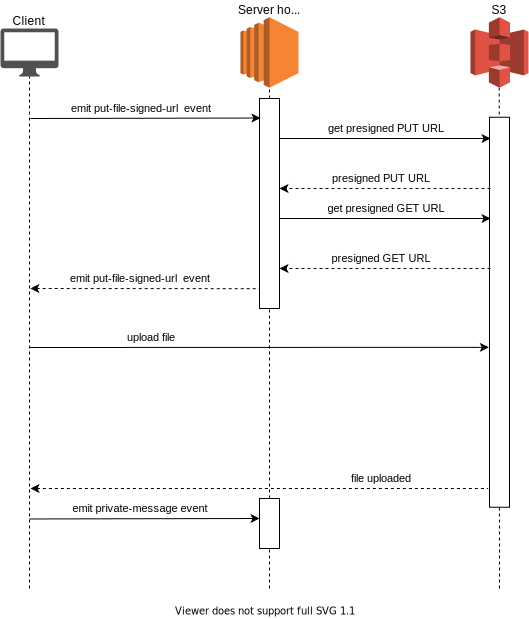
\includegraphics[width=\textwidth,keepaspectratio]{images/backend/upload-media.pdf}
	\caption{Interactions necessary for uploading media.}
	\label{figure:backend-stage-server-media-message}
\end{figure}

As seen from the diagram, the client uploads the file directly to S3. In order to do so, the client first asks the backend server for a presigned PUT URL, used for uploading the photo, and a presigned GET URL, which is valid only for a day and used later in order to send the message in the chat. Had I learned about Cognito Identity before doing this it could have been done differently, the client could get authorization credentials straight from Cognito and the entire communication with the server before uploading the file would be omitted.

\subsection{Securing messages}

For securing plain text messages, access to the API is granted only to those who are participants of a chat. First of all the JWT is verified and if valid then it is checked whether or not the participants of the chat include that user, if so then the user is authorized.

The media messages are stored in a private S3 bucket and they are not accessible to the public. For retrieving messages from a chat the server is asked to do so, the server then gets them from the API and presigns media messages' URLs after which the links to media are valid for one day (can be changed to any amount of time). Advantages are that, if the user wishes so, he can share the link to the media to non-participants of the chat. A disadvantage to this approach is that the server is involved, by the time I realized this could be done with a request to a HTTP triggered function the logic was already implemented.

\subsection{Using HTTPS}

Because there can be private data transported the server had to be secured.
The way I achieved the server to run over HTTPS is somewhat unexpected. Another way I think this could have been done is by getting a certificate authority\footnote{\href{https://en.wikipedia.org/wiki/Certificate\_authority}{https://en.wikipedia.org/wiki/Certificate\_authority}} such as Let's Encrypt\footnote{\href{https://letsencrypt.org/}{https://letsencrypt.org/}} to issue a digital certificate, use it to host a HTTPS server instead and add a DNS CNAME record to point to the EC2 instance hostname. However, this was achieved by using an Application Load Balancer\footnote{\href{https://aws.amazon.com/elasticloadbalancing/application-load-balancer/}{https://aws.amazon.com/elasticloadbalancing/application-load-balancer/}} as AWS provides communication over HTTPS to the load balancer. The load balancer essentially acts as a proxy server, as seen in Figure \ref{figure:backend-stage-server-https}. An advantage of doing this was that a load balancer needed to be set up for greater scalability anyway.

\begin{figure}[H]
	\centering
	
\includegraphics[width=.5\textwidth,keepaspectratio]{images/backend/server-proxy.pdf}
	\caption{How the ALB\footnote{Application Load Balancer} acts a TLS termination proxy\footnote{\href{https://en.wikipedia.org/wiki/TLS\_termination\_proxy}{https://en.wikipedia.org/wiki/TLS\_termination\_proxy}}}
	\label{figure:backend-stage-server-https}
\end{figure}


\section{REST API}

As seen and talked about in the architecture chapter the REST API is created from HTTP triggered AWS Lambda functions whose access are centralized by an AWS API Gateway, which essentially acts as a reverse proxy. For persisting the data I chose AWS DynamoDB\footnote{\href{https://aws.amazon.com/dynamodb/}{https://aws.amazon.com/dynamodb/}} as that is a managed solution as well.

\subsection{Project structure}

The file and directories hierarchy here is the easiest to understand compared to the other ones. The first four files/directories have been explained before. The \textit{serverless.yaml}  file is Serverless\footnote{\href{https://serverless.com/}{https://serverless.com/}} specific and contains IaC\footnote{Infrastructure as Code} that deploys all the necessary resources with their configurations, as talked about in the infrastructure chapter. The \textit{OPENAPI.yaml} file contains an API specification that makes it easier to describes and visualize the services providen by the \textbf{Think-In} API, it is written according to the OpenAPI Specification\footnote{\href{https://swagger.io/specification/}{https://swagger.io/specification/}}. The \textit{shared.ts} file contains code that is common across this application. In the last six directories every file corresponds to a HTTP triggered Lambda function. In the \textit{avatars} directory the \textit{post-avatar-token.ts} file contains logic that resizes and changes the user avatar when the user passes a token, i.e. when the user is logged in and changes his avatar from the profile page. The \textit{post-avatar-id.ts} file contains logic for handling the use case when the user picks an avatar when registering, at this point the user can't be logged in and therefore can't use a token to request to the function previously explained. The hacky solution I went through is that a user can change his avatar as long as he is unconfirmed and knows his ID. The \textit{translations} directory contains logic that deals with, of course, translation. For this I have relied the burden of translating between languages to Google Translate\footnote{\href{https://en.wikipedia.org/wiki/Google\_Translate}{https://en.wikipedia.org/wiki/Google\_Translate}} because it has always been my go-to language translation app. The function in the \textit{get-languages.ts} file simply returns the languages supported by Google Translate, the function in \textit{post-translate.ts} deals with actual language translation. The last four directories contain code for functions that respect the REST architectural style constraints.

\begin{figure}[H]
\begin{verbatim}
REST_API
|- tsconfig.json
|- .eslintrc.json
|- .prettierrc.yaml
|- node_modules/
|- serverless.yaml
|- OPENAPI.yaml
|- shared.ts
|- avatars/
   |- post-avatar-id.ts
   |- post-avatar-token.ts
|- translations/
   |- get-languages.ts
   |- post-translate.ts
|- chats/
|- notifications/
|- stages/
|- users/
\end{verbatim}
\caption{Backend server project structure.}
\label{figure:backend-stage-server-project-structure}
\end{figure}

\subsection{DynamoDB design}

Before further explaining we need to have a slight idea of how DynamoDB works. It is a NoSQL database that stores items in a table, each item containing attributes, this results in schemaless items very alike JSON\footnote{\href{https://www.json.org/json-en.html}{https://www.json.org/json-en.html}} objects. DynamoDB supports two types of primary keys:
\begin{itemize}
	\item \textbf{Partition key} - items are uniquely identified by a single attribute, based on the attribute the item will be assigned to a physical partition
	\item \textbf{Partition key and sort key} (composite key) - items are uniquely identified by a combination of two attributes, the items are assigned to a physical partition by the primary key, and are sorted in that partition by the sort key.
\end{itemize}

Having this knowledge I had to study the data access patterns of the application. One particular use case that stands out is fast message retrieval, most certainly if people used \textbf{Think-In} they exchanged only a couple messages and most importantly other contact data so further talking will be done through another medium. For this reason I don't want people to wait a long amount of time to retrieve that meaningful information. In order to achieve this I didn't want time to be lost on sorting the messages between users, so the fact that DynamoDB holds the data in memory naturally sorted helped, therefore I chose to have a \textbf{partition key} and a \textbf{sort key} where a message will have the following format:
\begin{itemize}
	\item Partition key of the format \verb|chat_{chatId}|
	\item Sort key of the format \verb|message_{timestamp}_{id}|.
\end{itemize}

In doing so, if we search by the partition key we get to the physical partition where the messages are stored sorted by timestamp, that sounds fast! The justification for an  additional ID at the end of the sort key is to account for the rare case where multiple messages have the same timestamp. Knowing that DynamoDB and the Lambda function are hosted in the Frankfurt region, I got an average response time of 281 milliseconds over 15 requests. The function was initialised (i.e. it had no cold start\footnote{\href{https://www.serverless.com/blog/keep-your-lambdas-warm}{https://www.serverless.com/blog/keep-your-lambdas-warm}}) before performing the requests. In case there was any doubt, the data identified by the partition key and sort key respects the contract of the message described in the frontend chapter.


Another data that needed to persist was notifications, that is who messaged a user while he was offline, next time he logs in he should be notified of the users who left him messages. In this case a notification has the partition key of format \verb|user_{userId}| and sort key \verb|notification_{id}|. An access pattern here would be to simply get all items that have the partition key equal to that of a user's ID in order to get all his notifications, whether or not the notifications are sorted doesn't matter. The contents stored for a notification is the message sender's information so next time the receiver logs in a new chat with the sender user will be loaded.

What is stored in the database is also information about stages, the information that can be seen in the horizontally scrolling area of the index page. In this case the partition key is \verb|stages| and the sort key is \verb|{stageId}|. The information stored about a stage is the following:
\begin{itemize}
	\item title - the stage title
	\item subheader - the text shown below the stage title
	\item body - description about the entity behind the stage
	\item externalLink - an external link to more information about the entity behind the stage
	\item imageLink - a link to an image provided by the entity behind the stage
	\item videoLink - a link to a video provided by the entity behind the stage.
\end{itemize}


In retrospective, after using other managed database solutions provided by other cloud platforms (e.g. Cloud Firestore, Firebase Realtime Database), interacting with DynamoDB hasn't been the most pleasant experience from a developer's point of view. For instance having to specify query expressions using strings did not feel modern to me. Moreover, performing pagination was a headache, the traditional limit and offset parameters have been substituted by  the partition key and sort key, so everytime I wanted to obtain another page I had to specify the last retrieved item's partition key and sort key.


\subsection{Changing avatar functionality}

At the heart of changing a user's avatar sits the function in Figure \ref{figure:backend-rest-api-avatar}. As observed by lines 2-3, in order to save bandwidth and improve loading times the image is processed so that it is resized, furthermore it's brought to a common format, in this case \verb|image/jpeg|. Between lines 5-12 the new avatar is uploaded to S3, and lines 14-20 change the \textit{picture} attribute of the user so that it now points to the newest location.


\begin{figure}[H]
\begin{lstlisting}[numbers=left,basicstyle=\small,language=JavaScript]
const uploadAvatarToS3AndUpdateUserAttribute = async (userId, avatarBuffer) => 
{
  const processedAvatar = await sharp(avatarBuffer)
                                  .resize(256, 256).jpeg().toBuffer();

  const { Location: avatarURI } = await s3
    .upload({
      Bucket: process.env.S3_CHATS_BUCKET!,
      Key: `avatars/${userId}.jpg`,
      Body: processedAvatar,
      ContentType: 'image/jpeg',
    })
    .promise();

  await cognitoIdentityServiceProvider
    .adminUpdateUserAttributes({
      UserPoolId: process.env.COGNITO_USER_POOL_ID!,
      Username: userId,
      UserAttributes: [{ Name: 'picture', Value: avatarURI }],
    })
    .promise();

  return avatarURI;
};
\end{lstlisting}
\caption{Logic of changing an avatar.}
\label{figure:backend-rest-api-avatar}
\end{figure}











    \chapter{Limitations and further improvements.}

Further development that can be done is towards scalability, for instance the application load balancer can be used together with Socket.IO Redis Adapter\footnote{\href{https://socket.io/docs/v4/redis-adapter/}{https://socket.io/docs/v4/redis-adapter/}} and multiple EC2 instances in order to accommodate for a larger amount of people using the application. More interactivity can be brought to the 3D stage, the fact that the attendee's can move their avatar around the stage serves a good basis for that.

If group chats are desired then a refactoring of the way chats are stored has to be made, currently a chat ID is calculated by hashing the ID of the user participants, which unless the chat is the global/stage chat the number of participants is always two.

An issue that can be more thoroughly analyzed is why sometimes requests to S3 from the frontend are unsuccessful. Several browsers claim it's a CORS\footnote{Cross-Origin Resource Sharing: \href{https://developer.mozilla.org/en-US/docs/Web/HTTP/CORS}{https://developer.mozilla.org/en-US/docs/Web/HTTP/CORS}} issue but I have configured the bucket such that CORS requests are allowed from any origin. What's weird is the inconsistency of the error, sometimes it works and sometimes it doesn't, on certain resources it works and on others it doesn't.
    
    \chapter*{Conclusions} 
\addcontentsline{toc}{chapter}{Conclusions}

As overall conclusions I have:

\begin{itemize}
	\item examined other implementations and studied their weak and strong points by using the applications that were free, after which I borrowed their strong points and improved their weak ones
	\item chosen the best available services and tools that fit to my use case in order to provide the best developer and user experience
	\item created an application that is straightforward to use and brought it into a working state into the real world, available to everyone on the internet, that includes acquiring and setting up a domain, setting up services and making them work together	
\end{itemize}
    \chapter*{Bibliography} 
\addcontentsline{toc}{chapter}{Bibliography}

\begin{itemize}
	\item \href{https://www.typescriptlang.org/docs/}{https://www.typescriptlang.org/docs/}
	\item \href{https://nextjs.org/}{https://nextjs.org/}
	\item \href{https://socket.io/}{https://socket.io/}
	\item \href{https://jamstack.org/}{https://jamstack.org/}
    \item \href{https://agilemanifesto.org/}{https://agilemanifesto.org/}
    \item \href{http://www.extremeprogramming.org/values.html}{http://www.extremeprogramming.org/values.html}
    \item \href{https://en.wikipedia.org/wiki/Extreme\_programming}{https://en.wikipedia.org/wiki/Extreme\_programming}
    \item \href{https://en.wikipedia.org/wiki/Software\_development}{https://en.wikipedia.org/wiki/Software\_development}
    \item \href{https://en.wikipedia.org/wiki/Waterfall\_model}{https://en.wikipedia.org/wiki/Waterfall\_model}
    \item \href{https://en.wikipedia.org/wiki/Infrastructure\_as\_code}{https://en.wikipedia.org/wiki/Infrastructure\_as\_code}
    \item \href{https://en.wikipedia.org/wiki/Event-driven\_programming}{https://en.wikipedia.org/wiki/Event-driven\_programming}
    \item \href{https://en.wikipedia.org/wiki/Representational\_state\_transfer}{https://en.wikipedia.org/wiki/Representational\_state\_transfer}
    \item \href{https://reactjs.org/docs/faq-structure.html}{https://reactjs.org/docs/faq-structure.html}
    \item \href{https://levelup.gitconnected.com/get-rid-of-relative-import-path-hell-in-your-typescript-project-9952adec2e84}{https://levelup.gitconnected.com/get-rid-of-relative-import-path-hell-in-your-typescript-project-9952adec2e84}
    \item \href{https://www.coreycleary.me/escaping-relative-path-hell}{https://www.coreycleary.me/escaping-relative-path-hell}
    \item \href{https://medium.com/@dan\_abramov/smart-and-dumb-components-7ca2f9a7c7d0}{https://medium.com/@dan\_abramov/smart-and-dumb-components-7ca2f9a7c7d0}
    \item \href{https://docs.aws.amazon.com/AmazonS3/latest/userguide/Welcome.html}{https://docs.aws.amazon.com/AmazonS3/latest/userguide/Welcome.html}
    \item \href{https://docs.aws.amazon.com/amazondynamodb/latest/developerguide/Introduction.html}{https://docs.aws.amazon.com/amazondynamodb/latest/developerguide/Introduction.html}
    \item \href{https://docs.aws.amazon.com/lambda/latest/dg/welcome.html}{https://docs.aws.amazon.com/lambda/latest/dg/welcome.html}
    \item \href{https://docs.aws.amazon.com/ses/latest/dg/Welcome.html}{https://docs.aws.amazon.com/ses/latest/dg/Welcome.html}
    \item \href{https://docs.aws.amazon.com/cognito/latest/developerguide/cognito-user-identity-pools.html}{https://docs.aws.amazon.com/cognito/latest/developerguide/cognito-user-identity-pools.html}
    \item \href{https://docs.aws.amazon.com/cognito/latest/developerguide/cognito-identity.html}{https://docs.aws.amazon.com/cognito/latest/developerguide/cognito-identity.html}
    \item \href{https://docs.aws.amazon.com/apigateway/latest/developerguide/welcome.html}{https://docs.aws.amazon.com/apigateway/latest/developerguide/welcome.html}
    \item \href{https://www.redhat.com/en/topics/api/what-does-an-api-gateway-do}{https://www.redhat.com/en/topics/api/what-does-an-api-gateway-do}
    \item \href{https://docs.aws.amazon.com/AWSEC2/latest/UserGuide/concepts.html}{https://docs.aws.amazon.com/AWSEC2/latest/UserGuide/concepts.html}
    \item \href{https://docs.aws.amazon.com/AmazonCloudFront/latest/DeveloperGuide/Introduction.html}{https://docs.aws.amazon.com/AmazonCloudFront/latest/DeveloperGuide/Introduction.html}
\end{itemize}
\end{document}
